% !TEX root = ./Report.tex
\documentclass{article}
\usepackage{graphicx}
\usepackage{subcaption}
\usepackage{caption}
\usepackage{color,soul}
\graphicspath{ {./Screenshots/} }
\title{ Kohonen Self Organizing Map- Project : 4 }
\author{Atsushi oba (s1230128),        Hitoshi Ikuta (m5221106) \\
   \and Chowdhury Md Intisar (m5212106),        Yunosuke Teshima (m5221151)
}

\begin{document}
\maketitle 
\section{Self Organizing Network}
  When a self-organizing network is used, an input vector is presented at
each step. The network tries to represent the input vector of higher dimention
to a lower dimentional space. Thus each new input tries to learn the parameter
to adapt. The best-known and most popular model of self-organizing networks is
the topology-preserving map proposed by Teuvo Kohonen, hence Kohonen self
organizing map. If an input space is to be processed by a neural network, the 
first issue of importance is the structure of this space.  Kohonen networks
learn to create maps of the input space in a self-organizing way. An image
below depicts the network learning the function f to map the input space to
output space. 

\begin{figure}
\centering
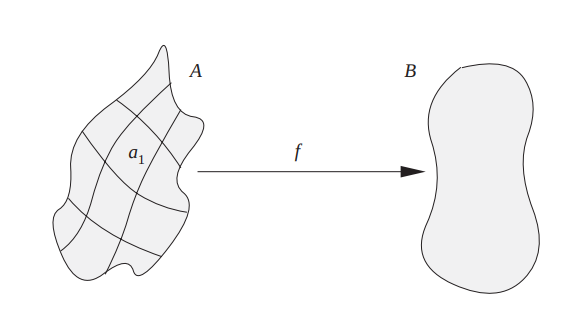
\includegraphics[width=.4\linewidth]{./simpleFunction.png}
\caption{Mapping of function from input space A to output space B. Here the
region \(a\) is selected.}
\end{figure}

\begin{figure}
\centering
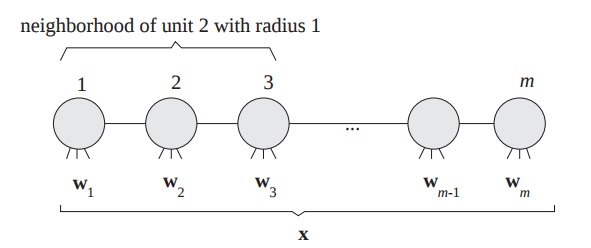
\includegraphics[width=.4\linewidth]{./learningAlgorithm.png}
\caption{Learning of the prototype}
\end{figure}






\section{Learning Algorithm}
 Let us consider, an n-dimensional space which will be mapped with the help of
 m-kohonen units or prototype vectors. Each unit becomes tne n-dimentional input
 x and computes the exciation or firing rate. The n-dimentional weights \(w_{1},
 w_{2},.., w_{m} \) are the computational neurons. The objective of each unit or
 neuron is that, it learns to specilize on different regions of input space.Thus
 when an input from such a region is fed into the network, the corresponding
 unit should fire with maximum excitation. During the training the unit which
 fires the most is selected using the winner takes it all algorithm. Then, the
 winner weight is updated as follows till it converges to the input. 

\begin{equation}
  \(w_{m}^{k+1} = w_{m} + \alpha(x - w_{m}^{k}) \)
\end{equation}

\begin{equation}
  \( w_{i} = w_{i} + \eta\phi(i,k)(\xi-w_{i}) \)
\end{equation}

Both of the equation 1 and equation 2 can be used to update the weights.
Equation 2 takes into amount its neighbour neurons. Thus a few neighborhood
function \(\xi(i,k\) have been introduced. In both equation \(\alpha and \eta\)
represents learning rate. 

\section{Output of the Program}

The given source code have been modified to take 150 samples of input from the
ULC machine learning repository. THe changes in the source code is attached as image.
The iris data set was fed into the program without any training label. The program have
 been run with different setting such as with different number of neurons, varied dimention 
of the input. Output depicted some interesting result showed in Table 1. 

\begin{table}[h!]
 \begin{center}
   \caption{The output of the program for different setting of M where M
   is the number of Neurons and  is the dimention}
    \begin{tabular}{l|r}
     \textbf{M} & \textbf{Accuracy}\\
     \hline
     3 & 66.66\% \\
     4 & 66.66\% \\
 \hl{5} & \hl{94}\% \\
     6 & 66.66\% \\
   \end{tabular}
 \end{center}
\end{table}

It is to be noted that, for each setting the program have been run for 5times
and the result have been averaged. Afer few iteration it was suprisingly
discovered that the program succesfully finds 3 clusters with high accuracy for
the value of \(M = 5\). For the other value of M the program results in only 2
clusters which result is accuracy of 66.66\%. Also, the weight initialization
part has been changed for convergance which is depicted in the Figure 3 and
Figure 4. After changing the distance function from normalized version of the
distance metrics we succesfully able to find 3 clusters.  


\begin{figure}
  \centering
  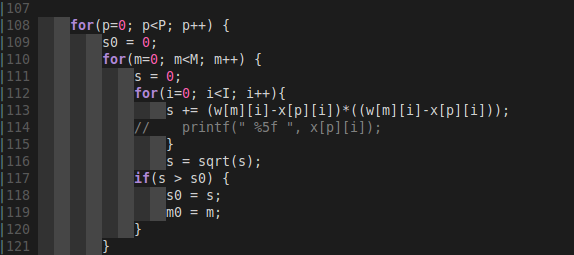
\includegraphics[width=6cm, height=5cm]{weight.png}
  \caption{Changed the distance metrics to Euclidean}
\end{figure}


\begin{figure}
  \centering
  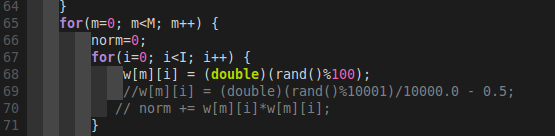
\includegraphics[width=6cm, height=5cm]{Random.png}
  \caption{Changed weight initialization}
\end{figure}

After we have changed the weight initialization method it resulted in early
convergence. 


\section{Research Findings}

\begin{itemize}
  \item The reason for failing to converge to 3 differnt cluster is due to the
initilization of the weight or prototype vector. 
   \item A good initialization can converge to proper number of  clusters easily.
   \item Another key factor is the \hl{dimention of prototype vector and the number
     of prototype vector}. 
\end{itemize}

Thus the above point greatly influence the outcome and convergence of the
prototype vector to the solution.




\end{document}


